\documentclass{beamer}
\usepackage{amsmath, amsfonts, graphicx}

\title{Surface Reconstruction Using the Level Set Method}

\author{Alexandre Vassalotti - \'{E}ric Renaud-Houde}
\begin{document}

\begin{frame}[plain]
  \titlepage
\end{frame}

\begin{frame}{Introduction 1}
Ultimate goal
\begin{itemize}
  \item Recreate a three dimensional surface from kinect data
  \item Depth map $\rightarrow$ Point cloud $\rightarrow$ Surface 
\end{itemize}
\end{frame}

\begin{frame}{Kinect}
Kinect characteristics:
\begin{itemize}
\item 640px by 480px color image (and infrared image if needed)
\item 640px by 480px depth map
\item 0.7m to 6m of depth range
\item Frame rate of 30 Hz
\end{itemize}
\end{frame}

\begin{frame}{Kinect Screenshots 1}
\begin{figure}[H]
  \centering
  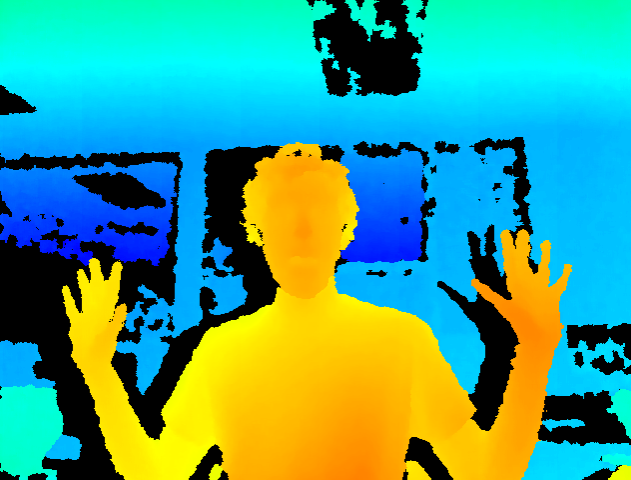
\includegraphics[width=0.7\textwidth]{img/depthmap.png}
  \end{figure}
\end{frame}

\begin{frame}{Kinect Screenshots 2}
  \begin{figure}[H]
  \centering
  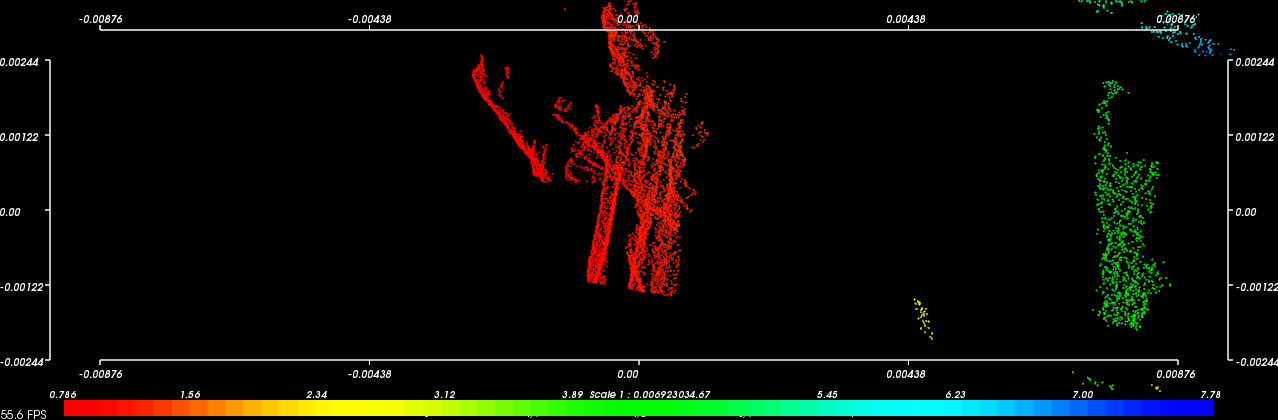
\includegraphics[width=0.7\textwidth]{img/pts.png}
  \end{figure}
  \begin{figure}[H]
  \centering
  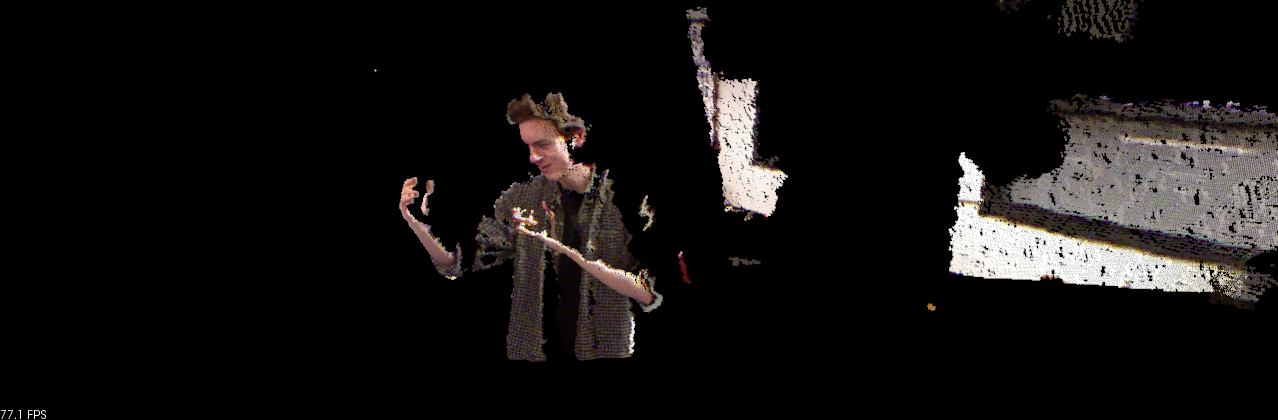
\includegraphics[width=0.7\textwidth]{img/pcl.png}
  \end{figure}
\end{frame}

\begin{frame}{Introduction 2}
  \begin{itemize}
  \item Reconstructing a surface from an unorganized dataset of points, how can we deal with:
  \begin{enumerate}
    \item Complex topologies (and topological changes)
    \item Noise in the data
  \end{enumerate}
  % orientation matters
  % cant assume white noise 
  \item Why? Point cloud information is incomplete. We want a useful 3d model.
  \end{itemize}
\end{frame}

\begin{frame}{Different approaches}
  Many techniques are used for surface reconstruction.
  \begin{itemize} %example
  \item \textbf{Explicit surface} %describes the precise location of a surface
  \begin{enumerate}
    \item Voronoi diagrams
    \item Delaunay triangulations
  \end{enumerate}
  \item \textbf{Implicit surface} %describes a particular isocontour of a scalar field
  \begin{enumerate}
    \item Poisson reconstruction
    \item Level Set Method
  \end{enumerate}
  \end{itemize}
\end{frame}

\begin{frame}{Level Set Method}
Definitions
\begin{itemize}
\item $\mathcal{S}$ : Data set of points.
\item $\Gamma$ : Level set (2d curve or 3d surface).
\item $\phi$ : Implicit level set function, the evolving higher dimensional interface 
\end{itemize}

\[
\Gamma(t) = \{\mathbf{x} \; | \; \phi(\mathbf{x},t) = 0\}
\]
\end{frame}
\begin{frame}{Visual representation}
\begin{figure}[H]
\centering

\includegraphics[width=0.2\textwidth]{img/Signed_distance2.png}
\end{figure}
\end{frame}
\begin{frame}{Iterative update}
Surface motion equation for $\phi$ (initial value formulation)
\begin{align}
    \frac{\partial \phi}{\partial t} + F \|\nabla \phi\| &= 0 \\
    \frac{\phi^{t+1} - \phi^{t}}{\Delta t} &=  -F \|\nabla \phi\| \\
    \phi^{t+1} &= \phi^{t} - \Delta t \; F \|\nabla \phi\| 
\end{align}
\end{frame}

\begin{frame}{Forces governing surface evolution}
How do we define $F$? \footnote{Fast Surface Reconstruction [...] - Hong-Kai Zhao - Eq.6}
\[
F = \nabla d(\mathbf{x}) \cdot \frac{\nabla \phi}{\| \nabla \phi \|}
+ d(\mathbf{x}) \cdot (\nabla \cdot \frac{\nabla \phi}{\| \nabla \phi \|} )
\]
\end{frame}

\begin{frame}{Energy Functional}
Where does this force formulation comes from? Derived from energy functional $E(\Gamma)$.
\begin{itemize}
\item Quantifies how $\Gamma$ corresponds to the data set
\item Has two global minima: $\Gamma = \Gamma_0$  and $\Gamma = \emptyset$.
\end{itemize}
It can be shown that the minimizer of the functional satisfies:
\[
\nabla d(\mathbf{x}) \cdot \mathbf{N} + d(\mathbf{x}) \cdot \kappa = 0
\]
\end{frame}
\begin{frame}{Visually}
\begin{itemize}
\item attraction to data points
\item surface tension
\end{itemize}
\begin{figure}[H]
\centering
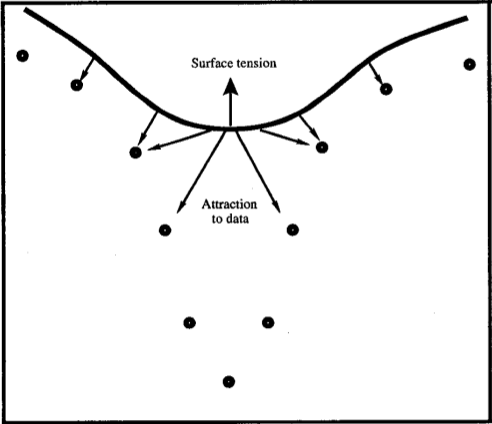
\includegraphics[width=40mm]{img/savadjiev3_3.png}
\end{figure}\footnote{Surface recovery from 3d point data - P. Sadavadjiev}
\end{frame}

% \paragraph{Gradient}
% \begin{itemize}
% \item central differences
% \item upwind scheme
% \end{itemize}

\begin{frame}{Optimizations?}
  Narrow Band Level Set Method \footnote{Adalsteinsson and Sethian, A Fast Level Set Method for Propagating Interfaces}
  \begin{figure}[H]
  \centering
  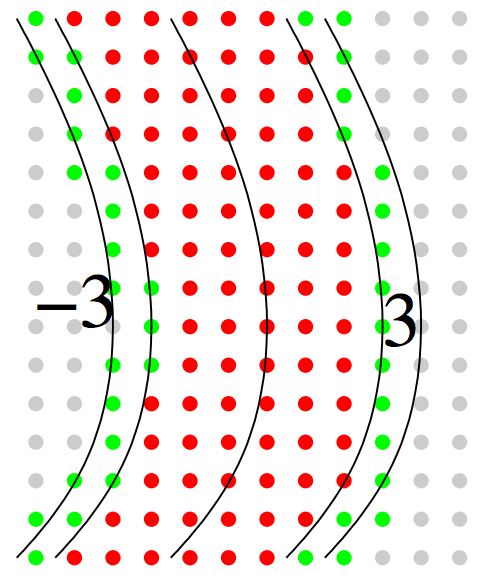
\includegraphics[width=0.2\textwidth]{img/narrow_band.png}
  \end{figure}
  \begin{itemize}
  \item Restrict the computations to a thin band around the level set
  \end{itemize}
\end{frame}

\begin{frame}{Experimental Results}

\end{frame}

\begin{frame}{Problems with this method}
  \begin{itemize}
  \item Extra dimensions affect computation time
  \item Dependence on grid precision
  \end{itemize}
\end{frame}

\begin{frame}{Questions?}
  
\end{frame}

\end{document}
